\documentclass[conference]{IEEEtran}
% Some Computer Society conferences also require the compsoc mode option,
% but others use the standard conference format.
%
% If IEEEtran.cls has not been installed into the LaTeX system files,
% manually specify the path to it like:
% \documentclass[conference]{../sty/IEEEtran}


% *** CITATION PACKAGES ***
%
\usepackage{cite}


% *** GRAPHICS RELATED PACKAGES ***
%
\ifCLASSINFOpdf
  \usepackage[pdftex]{graphicx}
  % declare the path(s) where your graphic files are
  \graphicspath{{../pdf/}{../jpeg/}}
  % and their extensions so you won't have to specify these with
  % every instance of \includegraphics
  \DeclareGraphicsExtensions{.pdf,.jpeg,.png}
\else
  % or other class option (dvipsone, dvipdf, if not using dvips). graphicx
  % will default to the driver specified in the system graphics.cfg if no
  % driver is specified.
  \usepackage[dvips]{graphicx}
  % declare the path(s) where your graphic files are
  \graphicspath{{../eps/}}
  % and their extensions so you won't have to specify these with
  % every instance of \includegraphics
  \DeclareGraphicsExtensions{.eps}
\fi

% *** MATH PACKAGES ***
%
\usepackage{amsmath}


% *** SUBFIGURE PACKAGES ***
\ifCLASSOPTIONcompsoc
  \usepackage[caption=false,font=normalsize,labelfont=sf,textfont=sf]{subfig}
\else
  \usepackage[caption=false,font=footnotesize]{subfig}
\fi

% *** PDF, URL AND HYPERLINK PACKAGES ***
%
\usepackage{url}

% correct bad hyphenation here
\hyphenation{}


\begin{document}
% Title ideas here:

\title{Exploiting the Social Graph: Increasing Engagement via
  Collaborative Interactive Evolution}
% Changed again to "via" - JJ
% I dont get it, we exploit the graph in order to increase user engagement in CIE
% By via, I understand that we use a CIE in order to encrease the engagment of users
% But I will leave it as you proposed I�m shure missing something

\author{\IEEEauthorblockN{Mario Garc\'ia-Valdez, Jos\'e Christian Romero, Alejandra Mancilla}
\IEEEauthorblockA{Instituto Tecnol\'ogico de Tijuana\\
Tijuana, Mexico\\
Email: (mario,amherag)@tectijuana.edu.mx,alejandra.mancilla@gmail.com}
\and
\IEEEauthorblockN{Juan Juli\'an Merelo Guerv\'os}
\IEEEauthorblockA{Universidad de Granada, CITIC\\
Email: jmerelo@geneura.ugr.es}
}

\maketitle


\begin{abstract}
Interactive evolution, where users' preferences guide the search, is
one of the leading techniques employed by Evolutionary Art
researchers. It is normally implemented as a web application to lower
the access threshold since it often depends on volunteers who visit
the system for fitness assignment. However,  several drawbacks limit
user participation: human fatigue and boredom result from evaluating 
a large number of phenotypes. To tackle these issues, in this paper we
propose an IEC system designed using a human-centered approach, with a
framework consisting of a social network of  
volunteers interacting with a population consisting also of a network 
of phenotypes, which also uses a graph model as a practical 
and efficient tool for mapping the relationships between actors and
objects in the system. A case study is presented as proof-of-concept, 
providing both conceptual and implementation details of a graph based model 
as it is  applied in the implementation of an IEC system. Our
experiments show that the data model can be successfully applied in a
gamification technique developed to increase user engagement, which
implies that this technique can successfully be used to 
decrease user fatigue and thus increase {\em performance} of the
interactive system.
\end{abstract}

% no keywords
\IEEEpeerreviewmaketitle



\section{Introduction}
Interactive Evolutionary Algorithms (IEAs) are, in general, standard EAs whose
fitness evaluations are performed by persons within an interactive 
system \cite{eiben2015interactive}.  Thus, the main evolutionary loop needs the intervention of a
human to perform the quality assessment of each proposed solution.
These kind of IEAs have demonstrated their ability for effectively
producing art and design \cite{Bentley:1999:intro,Sims:1991,todd:1992},
as well as other products in many other domains \cite{ie1}, and this
success has led to the development of web based systems such as \cite{picbreeder},
who depend on volunteers who visit the system to interactively help
with the search, using both anonymous and registered users. This
volunteer system lowers the requirements of anyone participating in
the experiment thus increasing the {\em performance}, in terms of {\em
  human brain cycles}, of the whole system.


However, the necessary intervention of humans in these systems leads
to them having several inherent drawbacks arising from the very nature of 
the algorithms, namely, the human fatigue caused by the interaction, and
the boredom arising when users evaluate a large number of phenotypes 
many of which are not interesting or are very similar to each other.


IEAs also share some of the issues commonly found in volunteer based systems
\cite{sarmenta2001volunteer,web:BOINC} such as the volunteer\'s lack of accountability,
and the need to build trust between participants and application providers. 
For the provider there is also the difficulty of establishing 
the amount of time and resources
a volunteer is willing to spend on the system, and how they decide if they
participate or not \cite{JJ:2016}. In order to increase participation and 
engagement, and to tackle the issues mentioned above,  
IEAs must follow a human centered design \cite{greenhouse2012human}, % reference and explain what
                                % you mean by that. It's an EC
                                % conference - JJ
                                % I explain more later in other section, with references, maybe move that to here? -Mario
                                % If not I will add a few words later, such a large topic -Mario
                                % even with a Journal:
                                % http://hcis-journal.springeropen.com/about
% a reference here would do no harm - JJ
giving extensive attention 
to volunteer users, not only because their
explicit evaluation is essential, but also because the context of the 
interaction affects the system as a whole. Users interact not only with the graphical
interface, and each phenotype, there is also the interaction
with other users, their previous evaluations and their own stream of activities
and past experiences. Thus users in the method presented in this paper are defined as dynamic entities 
interacting with an evolutionary computation having the fundamental purpose 
of evaluating phenotypes according to their preferences,
both explicitly or implicitly. 

In this work we propose giving the same
importance to users and their interactions as the population of 
phenotypes have in a traditional EA, even to the extent of using this
knowledge as an integral part of the evolutionary algorithm.
Instead of letting the user assign fitness directly via a rating
or selection system, fitness assignment could depend on the actions of
a group of users, possibly connected in a social network, and depend on how 
they tag, share, rate, or even delete the phenotype. The selection of parents could
also depend on the previous actions, leveraging information such as the fact that  they have the same tag, or shared by
similar users, or whether a leader of opinion liked both or if they are stored in the same collection.
That knowledge could also be applied in choosing which phenotypes would be presented to a
user, in order to give them those they will find more interesting or useful. 

We argue also
that a graph model is a viable representation for the above relationships and
interactions and can then be used to model and use, within the
evolutionary algorithm, actions performed by every user, which, as
mentioned above, will be used to assign fitness to solutions. Graph based
models are currently used in social networks to keep track  
of user interactions with media objects, places, and other users. Users of
social networks (for instance the Facebook Graph) are accustomed to express these 
complex relationships in sentences such as: ``John and Ann eating breakfast at Tony's''. 
Other example is the W3C Activity Streams 2.0 specification used for representing activities 
common in social web applications \cite{json:streams}.


When considering the type of relationships found in a genetic algorithm 
we can think of the Parent-Child relationship between a pair of parent solutions and
the child solution they produce. In IEAs there could be more entities involved, with 
even more types of interaction:


\begin{itemize}

  \item {\bf Phenotype-Phenotype} The parent-child relationship between phenotypes in the
  population, as mentioned before.  
             % do you mean different generations? Would be better to
             % make this more precise - JJ
  This relationships are naturally expressed as a tree.
  %, or a graph when both ancestors 
  %and descendants are considered. 
  Other semantic relations can also be
  of interest, 
  for instance the similarity relation between two phenotypes, could be used to measure
  the population's diversity.   %This is interesting for
                                %what reason? What do you mean by
                                %composition? "to be composed of"? - JJ
                                % Yes, I was thinking about collections as candidate solutions,
                                % but maybe not yet.
                                


  \item {\bf User-Phenotype} There are many kind of relationships
    between users and phenotypes, and these can be
  expressed using common actions found in social networks;
  as mentioned before.
  %for instance: share, like, rate or add to collection 
  %\cite{Prodromou:16:AS}. This was the Activity Stream referenced before. - Mario
    
  In IEAs these
  relationships are used to assign a single or a collection of
  fitness values to phenotypes \cite{garcia2013evospace}.   % I am
                                % afraid that individual is too
                                % similar to user, and you might get
                                % lost here. Maybe talk about
                                % "genotypes" or "phenotypes"? - JJ
                                % changed to phenotypes 
                                % do you think an additional
                                % explanation is needed? -Mario
  % Maybe explain that phenotypes are the expression of solutions
  % stored in the population, but do that above - JJ

  \item {\bf User-User}
  Relationship between users in an interactive evolutionary algorithm can also be modeled 
  as a social network, with well established semantics, algorithms and metrics \cite{ahuja1993network}.
  A graph model could enable researchers to find other ways of identifying leaders of 
  opinion or measuring the similarity between user's preferences. 
  These measures can then be used by recommender algorithms selecting 
  phenotypes according users' preferences. 

\end{itemize}
% Maybe this paragraph is somewhat redundant, 
% I think your point in the comments below is:
% so what if they are easily expressed as a network, thats not the main reason.
% if this is so, agreed. I will remove it- 
%These relations are naturally mapped to graphs, %They are bipartite
                                %graphs, but I don't see your point...
% Besides, _any_ relation can be mapped to a graph - JJ
%while other actions and 
%properties can also be modeled as a semantic network using
%basic subject–-predicate-–object expressions
%\%cite{Prud'hommeaux:14:RT}. % that's a graph, too.. - JJ
%Another reason for using a graph model % But for what exactly? A
                                % bipartite graph to express which
                                % relations? - JJ
%is the wealth of tools available for
%implementing and query the model, and the increased performance of
%native graph database systems \cite{holzschuher2013performance,holzschuher2016querying}.
 
A case study is presented as a proof of concept, providing both
conceptual and implementation details of a graph data model applied in the 
implementation of an IEA. The experiment was implemented using
the EvoSpace-Interactive framework \cite{garcia2013evospace}, and consisted of a web application
for evolving artistic drawings. The graph database is then used to
measure the degree of relationship between users and their participation.  

The remainder of this paper is organized as follows.
Section \ref{sec:interactive} presents related work on the topic 
of Interactive Evolution.
Then, Section \ref{sec:evospace-i} presents the computational platform on which 
the main proposal of this work is developed. The proposed graph model is 
presented in Section \ref{sec:HCF}.
The experimental work and results are presented in Section \ref{sec:experiments}.
Finally, a concluding remarks are provided in Section \ref{sec:conclusions}.


\section{Related Work}
\label{sec:interactive}
% IEC 
% Collaborative
% Users - Volunteers - Engagement
% Too much data
% Relational MySQL, Key-Value, Mongo, Redis, Memcached
% Not well suited for certain relations.
% Graph DBs, Performance, Query Langs 
% Are they any good? 
% Titan, Neo4J

Up until now, IEC  has been used in a wide variety of applications and problem domains
and remains an active area of research. However, in this work, emphasis is given to IEAs 
implemented as volunteer based collaborative systems; where volunteers interact and evaluate 
an evolving population, thus guiding the search based on an aggregate of their subjective 
preferences. What follows is not intended as a comprehensive survey, only a review of 
the most relevant contributions to the present work, with special attention put in
data structures and data management requirements.

From the earlier works in the IEC field the notion of user collaboration in a natural way
has been proposed. A notable application was the Galapagos Project \cite{sims1997interactivity},
an exhibit in the Tokyo Multimedia Museum (1997--2000) were visitors interacted with images presented in 
twelve displays by selecting those they found most aesthetically interesting by standing on
step sensors in front of them. An early example of web based collaboration is the work by 
Langdon \cite{langdon:2004}, which evolved fractal representations of virtual creatures. It used a 
distributed EA using a global population stored on a central web server sending 
portions of the population to remote clients using JavaScript. Users evaluated phenotypes locally 
and returned to the server those they liked more, to be distributed over the web.
Similarly, Secretan et al. \cite{picbreeder} and Clune and Lipson \cite{forms} use web-based IEAs 
to evolve artistic artifacts using a generative encoding, compositional pattern producing networks.

In all these systems, the interactive process is captured by the
system and no special attention is lent to the process of capturing
and engaging users themselves. In some cases, the genetic lineage of each
phenotypes is presented in a graphical interface 
where users can visualize the relationships between them, and evolutionary operators used in
their creation; they also display information regarding users and
their collaborations.  Common control panels  show, for instance,  
interesting phenotypes ordered by categories, number of votes, and
best of the week among others. In a recent work by 
Wagy \& Bongard \cite{wagy2014collective} user interaction is needed for evaluating the fitness and developing
new designs of robot locomotion. Collaboration is encouraged by gamifying the system 
using the maximum distance indicator to inspire the user to try and ``beat�'' previous designs. 

Implementing recommendation algorithms or adding gamification techniques have the goal of encouraging participation 
but require the use of a database system for managing the additional data required. 
For example, Picbreeder \cite{picbreeder} is implemented with a service oriented
architecture using a relational database and the file system for genotypes and images. Other works employ the 
use of No SQL databases like the work of Seyama and Munetomo \cite{seyama2016development} where they
employ a Platform as-a Service (PaaS) and NoSQL database to facilitate the collaboration 
among a large number of users for the interactive modeling of 3D glasses.  This system reduces the user fatigue
by using a collaborative filtering algorithm to show only the
information utilized by similar users. In any case, using gamification
techniques imply that we must deal with interactive evolutionary
system as socio-technical constructs, where the social aspects are
essential to understand its dynamics. In this sense, conclusions
reached with other systems such as NodEO
\cite{DBLP:conf/gecco/MereloCGCRV16} can also be applied to this
system; and applying social network techniques such as graph analysis
to their study will allow us to understand them more thoroughly. 

Collaborative IEC (C-IEC) systems also need to store highly connected data, as it is common in current applications
like social networks. In order to deal with large datasets of connected data found in these systems,
graph databases \cite{angles2012comparison} have been proposed as an alternative to relational databases 
which have performance limitations when dealing with highly connected data \cite{holzschuher2013performance}.
In this work the use of a graph data model for representing the interactive process of C-IEC systems is proposed.
Moreover, an proof-of-concept implementation of an IEA incorporating the graph model is presented.

\section{Experimental setup: the EvoSpace-Interactive framework}
\label{sec:evospace-i}
\begin{figure}[!t]
    \centering
        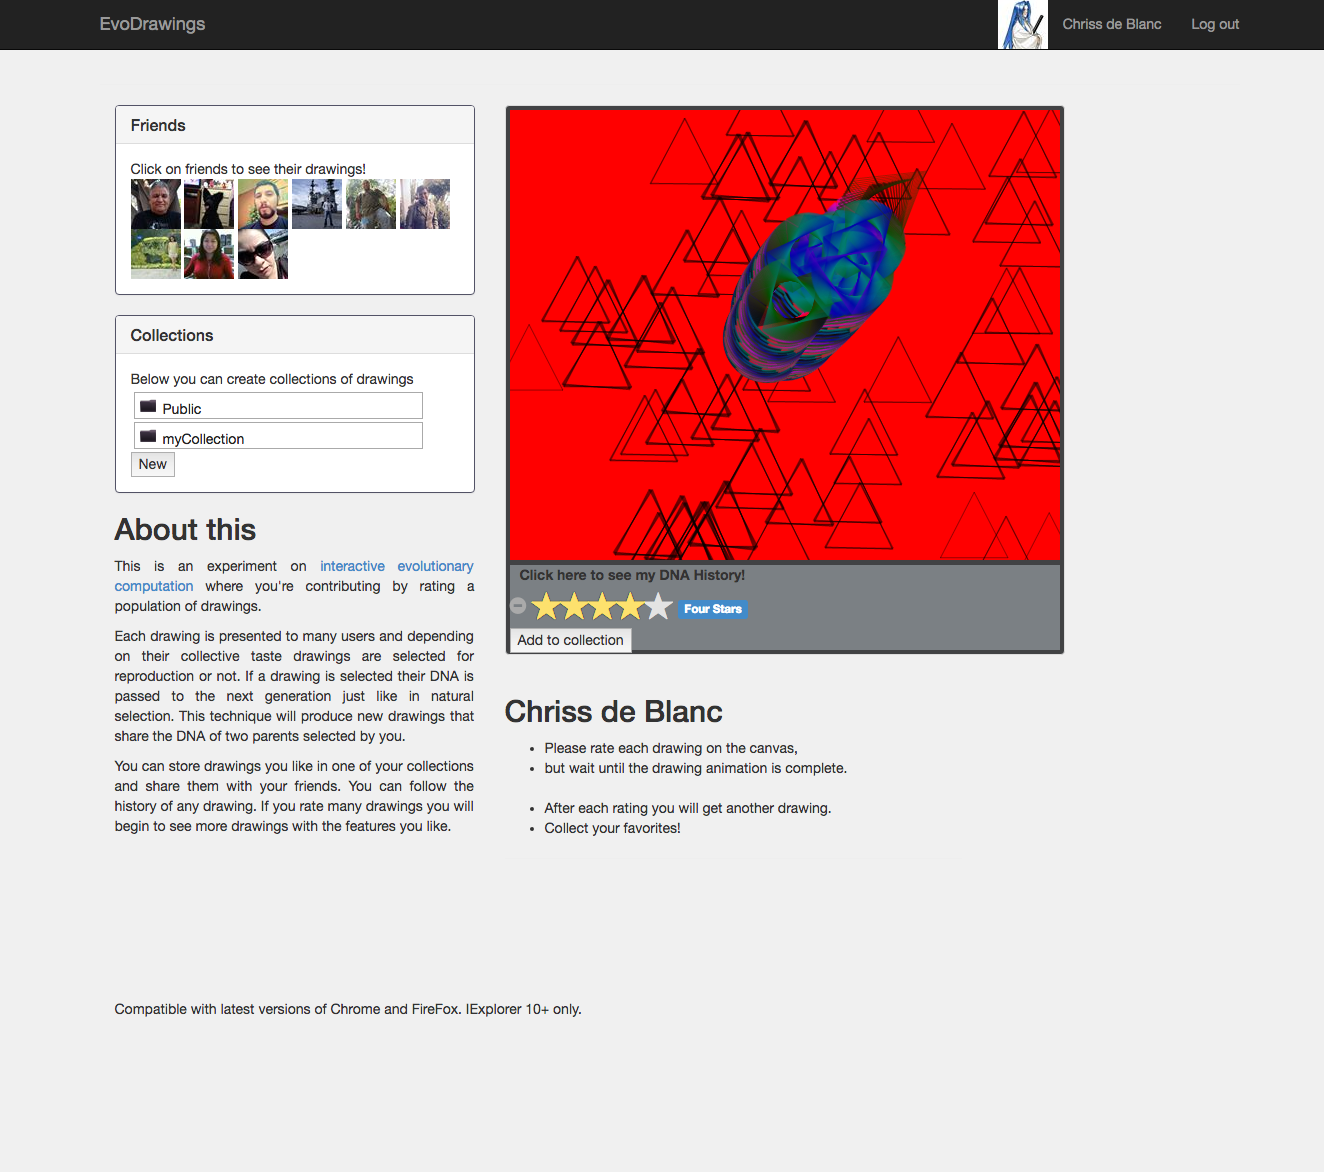
\includegraphics[width=3.5in]{img/UI_ed01.png}
    \caption{User interface of an EvoSpace-Interactive application.}
    \label{fig:web}
\end{figure}

As a case study, a IEA was developed using the 
EvoSpace-Interactive (ES-I) platform \cite{garcia2013evospace}
A brief description of the application is presented next, focusing
on the data elements that where ported to the graph model.

\subsection{Fitness Assignment}
\label{sec:assignment}
The ES-I platform employs a collaborative technique,
where several registered users assign a quality assessment to a single
phenotypes and then an aggregated fitness value is calculated. The fitness
assigned to each phenotypes depends on the taste of each particular user, 
resulting in a many-to-many relationship between users and phenotypes. 
Many systems query this user-phenotype relation to extract relevant
knowledge about the process and the population, for instance showing the
most popular phenotype, or the the user with more participation 
\cite{picbreeder}.
In order to do this, data about phenotypes 
must be permanently stored, even
if they are no longer in the active population. 

\subsection{Collaboration}
\label{sec:col}
After entering the web application by using their Facebook account,
users can collaborate with their Facebook friends, 
sharing those phenotypes they like, or by taking phenotypes
from their friend's collections by using the web interface depicted 
in Figure \ref{fig:web}.
At the top left corner a list of Facebook friends is presented
to encourage users to interact with the system. In the central 
\emph{ Wall } area, a phenotype sampled from the population that is
being evolved via the evolutionary algorithm 
is shown to the user.
Here, the user can interact with the system in two ways.
First, he can assign a quality assessment to the phenotype using
a five star rating system or,
additionally, a user can choose to add an image to one of their \emph{Collections}.
A collection is a special folder that stores those phenotypes a user likes and wishes
to save. After the user finishes interacting with the phenotype
on the Wall, he can choose to retrieve a new one from the population.
At the left hand side, the web page shows the \emph{Collections} section.
The user can create several collections, to group and organize his favorite 
artifacts. Moreover, users can browse the content of each collection and from
there share images through their social network.
When a user hovers the cursor over a phenotypes a pop-up pane shows how many users have
liked the phenotype. The pane also includes a link to the phenotype's 
details, the parents, genetic operators that created it, and genealogy
information. This makes the assignment of fitness through the rating
system a {\em social} activity, pursuing the objective of this work,
which is to increase engagement of the users.

\begin{figure*}[!t]
    \centering
        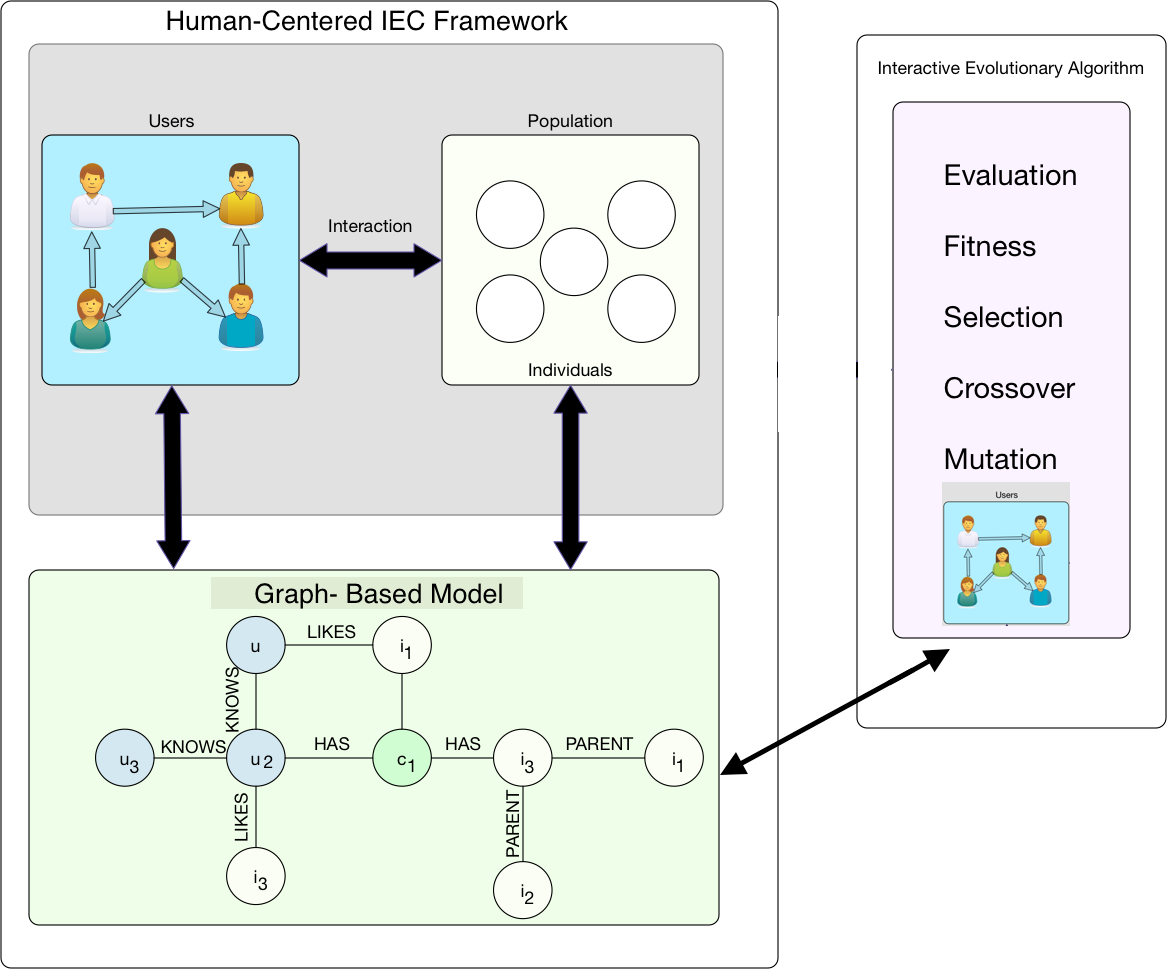
\includegraphics[width=3.5in]{img/framework.png}
    \caption{IEC Human-centered framework.}
    \label{fig:uc_framework}
\end{figure*}

\section{IEC Human-centered framework}
\label{sec:HCF}
The general goal of this research is to develop a human-centered \cite{gasson2003human} framework
for interactive evolutionary computation (IEC) in order to increase
participation and also to minimize the amount of evaluations needed for the
evolutionary process in a given IEC application. We deliberately use the 
more general
term Human instead of User, because humans are not always playing the role of
users in software engineering sense, they could just be interacting 
naturally with their environment and with out knowing they are implicitly
evaluating a possible solution. In other cases the evaluation could be done
by the natural interactions of a group of humans in a collaborative fashion
or not. For instance the IEC algorithm could be trying to optimize 
the design of an exit sign in an airport, then the quality of this sign could be
determined by the average time it takes a sample of people to 
find the exit. In this example there could be certain collaboration
between users if they are not traveling alone, but of course this is only one of
the considerations designers could make. 


The human centered framework consists of three high level components depicted
in figure \ref{fig:uc_framework}:
\begin{itemize}
  \item {\bf Interactive Evolutionary Computational system} 
  This is the real world system that we are going to represent in the model, 
  it consist of human users and their interactions with one or more phenotypes
  from
  the population. There are many ways in which humans could interact 
  with phenotypes, this could be through a mobile device, a user interface 
  or by interacting with real world objects generated as part of the algorithm 
  \cite{de2014artists,de2013unplugging}. 
  There is also the possibility that fitness or even part of the search 
  to be done by devices lent by the human \cite{DBLP:conf/gecco/MereloCGCRV16}.
  The information gathered through the interaction is the primary concern
  as it will guide the search. 

  \item {\bf IEC Data Model}
  A data model is used to describe the IEC system prior to a physical 
  implementation.  Depending on the domain several techniques can be used.
  Parts of the system could be better described by an Entity relationship 
  modeling to be used in a relational database or a class digram for a 
  key-value store. 

  A graph is proposed for modeling the social network of users 
  and their interaction with the population. When implemented a graph database 
  will be the back-end of the system. This  backend will then be
  used by the EA and the user interface, in a Model-View-Controller architecture. 

  \item {\bf Evolutionary Algorithm} 
  The EA algorithm queries the graph model, and then updates those nodes that 
  are part of the population. The EA could also be done with the help of
  humans, for instance in the XY project \cite{de2013unplugging} artists physically created
  the new population.  
\end{itemize}


%These components will be described in detail next.
% Besides, add something about the innovation in this paper, for
% instance, explaining that the data model is extended to a graph here
% - JJ

%Ok, I hope is not to much. Please edit at will - Mario

Besides, the methodology presented in this paper for interactive
evolutionary computation is a proposal to frame it as human centered computing \cite{sebe2010human},
in which the context, environment, interfaces, preferences, accessibility, human relations, cognitive
limitations, culture, creativity and other human aspects are an integral part of the system. 
This view requires a multidisciplinary approach, as well as multiple
knowledge representation formalisms. 
As a first step forward, the traditional data model is extended with a graph, in order to have 
yet another view to exploit. In the following section a description of
the data model is presented. 

\section{IEC Graph Data Model} 

A graph is composed of two fundamental entities: nodes and edges,
both having attributes. Nodes are abstractions of the objects in the real 
world system, and relationships describe their interactions. Types describe
the attributes describing an entity, and edges express relationships
between nodes. 

As it was mentioned before, an IEA must be modeled considering the 
entities involved in the interaction, if we consider the EvoSpace-Interactive framework
described in section  \ref{sec:evospace-i} we could find the following types of
nodes and relationships:

%Next we describe the types of nodes and
%relationships in the system. % I think a bit of more explanation would
                             % help why you have these types and
                             % whether they are simple implementation
                             % details or part of the method - JJ
                             % Explaining above, the graph will depend on the elements of the interaction - Mario


\subsection{Node Types}
\begin{itemize}

\item {\bf Users} This type of node represent the human users of the system and have 
the following attributes: {\tt id} a unique identifier, {\tt name}  and {\tt created}
specifying the  creation date (time stamp) of the node. 

\item {\bf Phenotype} This type of node has the following attributes: 
{\tt id}, {\tt chromosome}  and {\tt views}, which is the number of
times users have seen or interacted with this phenotype and, finally, 
 {\tt created}, the time and date of creation as above..

\item {\bf Collection} This type of node represents the collections belonging
to users, their attributes are {\tt id}, 
{\tt name}, {\tt created} and {\tt is\_private} indicating if contents
belonging to this collection can be shared with others. Collections can contain
phenotypes and a single phenotype could be shared by many
collections. % This is why they are not attributes - Mario
% You can simply have an attribute that is a list of the collections
% it belongs to - JJ
% Right, but:
%  1) The relationship could have additional atributes, (when it was stored, order, etc.)
%  2) Then it could be difficult to query with Cypher (I think) -
%  Mario
% Then it's more of an implementation detail, but anyway, point taken
% - JJ
\end{itemize}

The interaction between these entities and how they are represented by relationships 
between nodes are presented in the next subsection. 

\subsection{Relationship Types}

These relationships are expressed as edges in the graph. We use
several of them.

\begin{itemize}
\item {\bf Likes} This relation describes the interaction between a user and
a phenotype in which a rating value is assigned this is represented by 
the {\tt rate} attribute. In the current application a user is allowed to rate
a phenotype multiple times, so the date of the interactions is also of
interest.

\item {\bf Knows} The relation connects two users that know each
other. 

\item {\bf Parent} Describes what phenotype is the parent of a new
  phenotype. 

\item {\bf Has} The relation describes an ownership relation between users and
those collections they own. Also a collection {\tt has}  phenotypes stored
in them.
% In figure \ref{fig:has} the {\tt has} relationship 
% between certain nodes $user$, $phenotype$ and $collection$ is shown.

\item {\bf Shared} When a user takes an phenotype from a friend's collection, this interactions 
is described by a {\tt share} relationship between the user and the
phenotype.  % Still think that user and individual is confusing - JJ
            % Agreed corrected -Mario
            % I was thinking about calling them Solutions or Candidate
            % Solutions,
% Solutions is OK, but also phenotype - JJ

\item {\bf Saved} When a user takes an phenotype from the wall interface, this 
interactions is described by a {\tt save} relationship. 
\end{itemize}

  
% \begin{figure}[!t]
%     \centering
%         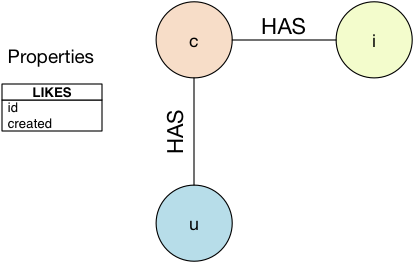
\includegraphics[width=2.5in]{img/edge_properties_has.png}
%     \caption{ The {\tt has} relationship type example and attributes.}
%     \label{fig:has}
% \end{figure}

Is important to notice that this model is still a partial view of the IEC system,
and other models can could be used in practice when implementing the
system. % It is also a bipartite graph, which could be converted to a
% single-party graph with only one type of node. 
% I don't get this comment, yes some relations are bipartite, but If we see the whole
% graph I think is a multi-graph.   - Mario 
% I will check the  single-party graph conversion you suggest, I don't
% know the concept. - Mario
% Does not matter much... it converts a bipartite graph to another
% graph with a single kind of nodes, phenotypes or users, for instance
% - JJ
%
% I don't think "collections" should be nodes too. They are simply
% attributes for an individual - JJ
% They are nodes, I added the reason above. - Mario
For instance a relational database was used for the implementation of a 
basic user profile and authentication module. Also the active population 
was kept in a key-value store in memory for performance reasons.  
Nevertheless, having a multi-model implementation can give important 
insights of the behavior of the system. This architecture was validated
by a case study, requiring the interaction of all of the components.        

\section{Case Study}
\label{sec:experiments}

We present in this section the results of a comparison between three versions
of the same IEC application. The goal of the experiment is to compare two 
gamification techniques to increase volunteer participation against a third 
without any technique applied.

The main difference between both versions employing gamification is how the fitness of phenotypes
is calculated and the information presented to users. 

\subsection{Gamification techniques}
\label{sec:gamification}

%This section on gamification should go to the intro and state of the
%art, since it is one of the main points of the paper - JJ
Gamification is defined by Deterding et al. as
``the use of game design elements in non-game contexts'' \cite{deterding2011game}.
The gamification element employed in this work is rewarding mechanism 
\cite{dubois2013understanding}, in general they consisting of a reputation systems with score points, 
levels and leader boards. Points are awarded to users in response of
the accomplishment of certain activities that need to be encouraged. Levels depend
on the score and certain features of the game are only available to gamers when 
they reach a giving level.

The rewarding mechanism as it is applied in these versions 
consists in giving more importance to the preference of those users having a higher reputation
as given by the score points and experience levels.  

The score achieved by users depends on the actions he does in the system as
each time a user does one of these actions their score is incremented by one:
\begin{itemize}
\item Start a session.
\item Rate a phenotype.
\item Create a collection.
\item Save a phenotype of the wall to a collection.
\item Save a phenotypes from a friend's collection.
\item Explore collections of other friends.
\end{itemize}

Only the ``Start a session'' and ``Explore collections of other friends'' actions 
are not reflected in the graph model since they are stored instead in the PostgreSQL relational
database system. This is because user sessions and authentication, as well as basic
web requests, are handled directly by the Django web framework \cite{garcia2013evospace}.  

Two scores are used to determine the weight of a user's preference:
\begin{itemize}
\item {\em Experience}: This value depends on the score and is a value 
between 0 and 100. It is assumed for this case, that once a user
reaches a 100 actions, it has enough experience on using the application.   

\item {\em Participation}: This value is simply the degree of the user node 
in the graph. This measure considers the number of users he knows,
collections and phenotypes rated.    
\end{itemize}

Three versions were compared:
\begin{itemize}
\item Base (B). All users have the same weight.
\item Non Graph Gamification (G). Only experience is considered
\item Graph Gamification (GG) . Both experience and participation are considered.
\end{itemize}
When gamification was employed, all score values known where presented to users
and a ranking of users by weight was shown in a window. A screen capture of
this interface is shown in figure \ref{fig:top-users}. 

\begin{figure}[!t]
    \centering
        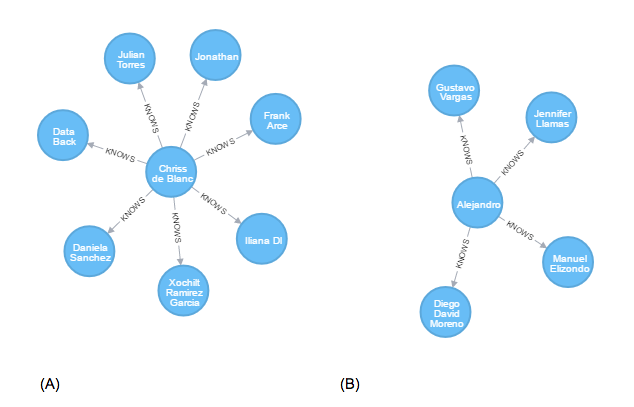
\includegraphics[width=3.5in]{img/users_known_1.png}
    \caption{Comparison of two users showing the {\tt knows} relationship.}
    \label{fig:users-graph}
\end{figure}



\begin{figure}[!t]
    \centering
        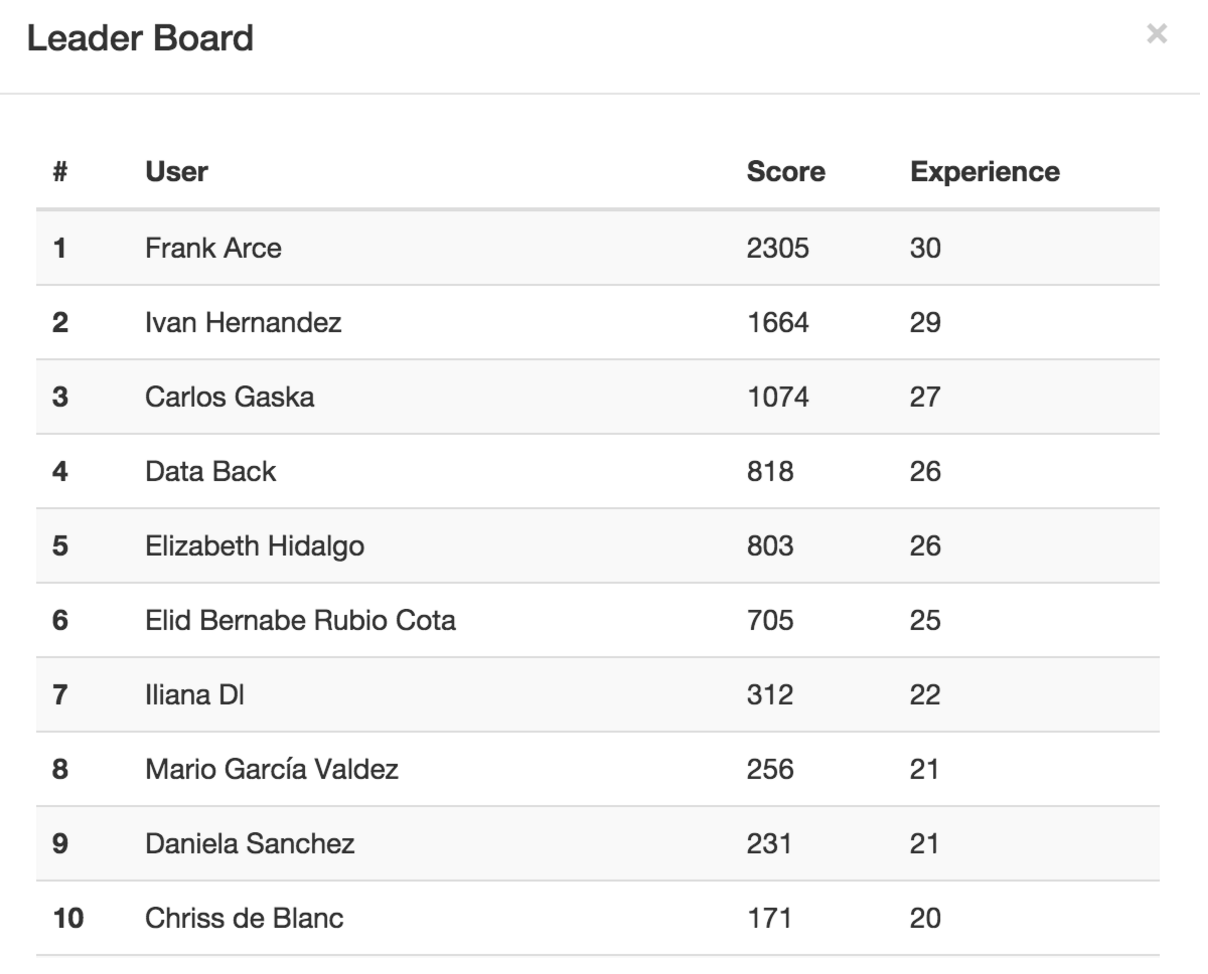
\includegraphics[width=3.5in]{img/leaderBoard.png}
    \caption{User interface showing top users.}
    \label{fig:top-users}
\end{figure}



\subsection{Set-up}
\label{sec:setup}

The three versions of the EvoDrawing web application were deployed to the
Heroku cloud service with the same configuration: using the
Heroku Free option with a 512 MB of RAM, adding only the GrapheneDB and RedisTOGO plug-ins.
Table \ref{tab:params} shows the parameters used for the evolutionary algorithm. The graph database 
system used in the implementation was Neo4J as it was already available as a plug-in in Heroku, is well documented
and a scalable solution \cite{miller2013graph,holzschuher2013performance}.  

\begin{table}
  \small
  \caption{ Parameters for experiments.  }
  \label{tab:params} 
  \centering
  \small
  \begin{tabular}{l  c   }
    \hline\noalign{\smallskip}
     Parameter & Value \\
    \noalign{\smallskip}\hline\noalign{\smallskip}
    Initial Population Size   & 80 \\ \hline
    Sample Size & 1 \\ \hline
    Step Size & 8 Samples \\ \hline
    Mutation &  \\ \hline
    Selection & Tournament \\ \hline
    Tournament Size &  6 \\ \hline
  \end{tabular}
\end{table}

% Anuncements
At the start of every experiment, a call to participation was issued
through social networks, 
particularly on Facebook and Twitter.
It is important to note that volunteers needed to log-in to Facebook and give permissions to the 
web application in order to participate, in this case there were no anonymous volunteers. This enabled the automatic access to
each participant's social network and enabled the system to store a local copy of those friends participating.
However, another experiment would be needed to see the effect this
requirement has on participation, since we are not dealing with it in
this paper. 

The link used in the call for participation
was shortened Google URL, that provides metadata and analytics for the
users that click on it. 
In table \ref{tab:urls} the URL for each deployment in the Heroku platform is shown,
along with the short URL and the analytics link. In the same table a link to the GitHub 
application repository used to deploy to Heroku is also listed.    

\begin{table}
  \small
  \caption{ Deployment data. URLs were {\tt
      evodrawings0(1,2,3).herokuapp.com}. For analytics URLs, add {\tt
    .info}.}
  \label{tab:urls} 
  \centering
  \small
  \begin{tabular}{l l l }
    \hline\noalign{\smallskip}
     Deployment &  Shortened URL &  Github Repository \\
    \noalign{\smallskip}\hline\noalign{\smallskip}
    B   & goo.gl/jLis4Q &  mariosky/evospace-js \\ \hline
    G   & goo.gl/jqjNy5 &  mariosky/evospace-js\\ \hline
    GG  & goo.gl/J8TCe1 &  mariosky/evospace-js \\ \hline
    \end{tabular}
\end{table}

Only data for the first week of deployment was considered for the experiments, and they where conducted 
between January and May of 2016. 

\subsection{Results}
\label{sec:results}

Before launch, each deployment was first tried with a few beta testers. When applying the leader board
gamification technique for the first time a problem was found in this stage. The problem was that some 
users were cheating by giving a rating to an animation even before it was returned from the server, this was done by just
constantly clicking the mouse button. This is a common problem found in systems using leader boards because
by making the scores visible to other players they are encouraged to compete \cite{hickman2010total}. 
According to \cite{kumar2013gamification} best-practice gamification designs try to
refrain from using this element because of  problematic consequences of competition, which can result 
in negative conduct, low cooperation and collaboration, or disadvantaging certain player
demographics such as women. In order to still measure the effect of the leader board on the system, the 
problem of cheating was mitigated by disabling the rate button for a certain amount of time giving the animation
enough time to finish. But the problem persists, competitive users will try to get in to the leader board by other means.

The results of each of the three experiments in terms of participation are detailed next.

\subsubsection{ Base deployment}
After a week of the announcement the total number of volunteers for this experiment was 53 registered users. 
The total number of nodes generated in the graph was 595, with a total of 2220 relationships. In this
experiment a total of 500 new phenotypes where generated. The total number of evaluated
phenotypes for each volunteer is presented in figure
\ref{fig:top-ranked-participation} in blue. Users are ranked by
the number of phenotypes they rated, in the \emph{x} axis is the rank, and in the \emph{y} axis 
the number of phenotypes evaluated using a logarithmic scale.   % Ranked by... - JJ
% Done - Mario


\subsubsection{ Non Graph Gamification deployment}
The total number of volunteers for this experiment was very close to
the one obtained in the previous
experiment: 54 registered users. The total number of nodes generated in the graph was 648, 
with a total of 2596 relationships. These numbers are close to those obtained in the base experiment,
with a marginal increase in participation. The increased participation also helped in the creation of
more phenotypes for a total of 648. The total number of evaluated
phenotypes for each volunteer is presented in figure \ref{fig:top-ranked-participation} in red. 

\subsubsection{ Graph Gamification deployment}
This experiment had the higher number of volunteers for for a total of 68 registered users. 
In this experiment a total of 3594 new phenotypes where generated in the experiment. 
The total number of evaluated phenotypes for each volunteer is presented in figure 
\ref{fig:top-ranked-participation} in green. 

The results presented in figure \ref{fig:top-ranked-participation}, show that those users with
higher level of participation in deployments B and G, had about the same behavior, but the difference
came with users with medium level of participation, in this case participants where more engaged in deployment
G. When comparing all the experiments the deployment GG had the higher number of participation in users
of all levels.    

\begin{figure}[!t]
    \centering
        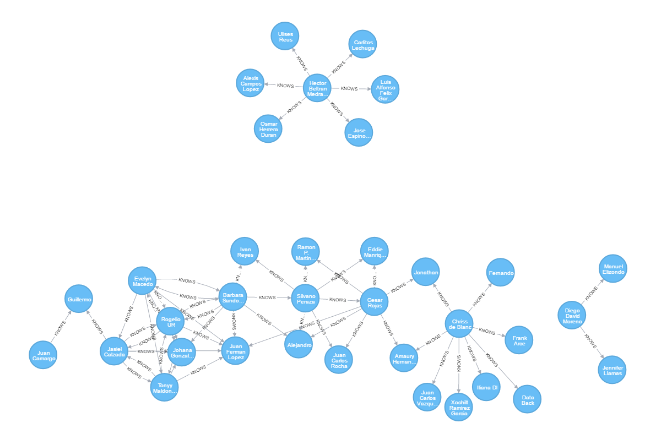
\includegraphics[width=3.5in]{img/user_known_2.png}
    \caption{User network view of the Base deployment}
    \label{fig:B-network}
\end{figure}
\begin{figure*}[!t]
    \centering
        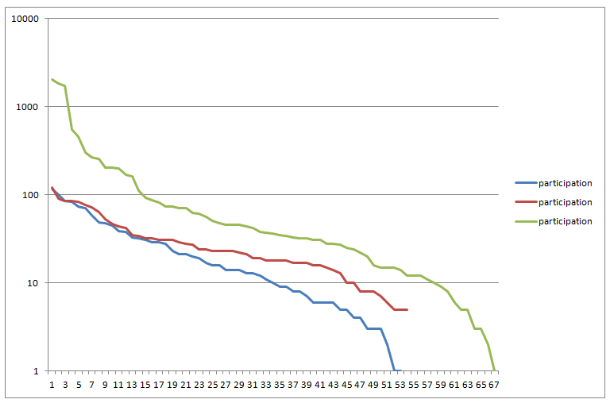
\includegraphics[width=5.3in]{img/comparison.png}
    \caption{Users ranked by the number of phenotypes they rated vs. the number of phenotypes evaluated using a logarithmic scale. } % Explain a little more and label axes. The
                         % three lines have the same label,
                         % "participation". Not too clear - JJ
                         % Done - Mario
    \label{fig:top-ranked-participation}
\end{figure*}

When monitoring the experiments by querying the graph database,  the Cypher query language 
provided interesting views on the data that it would have been
difficult to replicate with a relational database, for instance, to show the social network of volunteers 
as shown in figure \ref{fig:B-network}. 

The same can be applied to 
the population, or the interaction as a whole. The graph could be used also by the evolutionary
algorithm, for instance when creating a new phenotype 
parents could be selected only if there is a minimum distance between them in the graph.

\section{Conclusion}
\label{sec:conclusions}

% Using graphs improves engagement and also provides for a model for
% visualizing different experiments better. It has to tie with the
% initial objectives.

Collaborative and volunteer based IEC systems involve the dynamic 
interaction of many entities and artifacts. Employing a multi-model approach
can benefit researchers to understand and visualize this kind of systems better.
In this paper a graph model was proposed as a complement to current
models, initially to improve the visualization of different
experiments, but in this paper we prove that this model  enables
the implementation of a gamification technique to improve engagement in
a case study. Providing a common arena where users are aware of the
activities of other users in the social vicinity, as well as using
this graph to assign fitness allows in one hand for a greater
engagement by the users and from the algorithmic point of view a more
complex way of assigning fitness and push the generation of content
forward. 

One of the interesting future lines of work would be to look a bit
more closely at the behavior of users rating the system. These initial
experiments hint at a possible power law, which might indicate that
the IEC system could be self-organizing, a process that would allow it
to reach a critical state, as has been found in software repositories,
for instance \cite{Merelo2016:repomining}. The dynamics of this kind
of system are fundamentally different, and our future research will
include exploring these aspects of the system. Another line of work would be to study the negative effects of using 
gamification techniques to improve engagement, like cheating or competition.
Finally, the refinement of the proposed Human-Centered framework will need
more case studies and further multi-disciplinary research. 

\section*{Acknowledgment}

This work has been supported in part by: de Ministerio espa\~{n}ol de
Econom\'{\i}a y Competitividad under project TIN2014-56494-C4-3-P
(UGR-EPHEMECH). 

% trigger a \newpage just before the given reference
% number - used to balance the columns on the last page
% adjust value as needed - may need to be readjusted if
% the document is modified later
%\IEEEtriggeratref{8}
% The "triggered" command can be changed if desired:
%\IEEEtriggercmd{\enlargethispage{-5in}}

\bibliographystyle{IEEEtran}
\bibliography{../bib/evospace-i,../bib/volunteer,../bib/biblio,../bib/geneura}

\end{document}


\end{document}


